\ifx \globalmark \undefined %% This is default.
	\documentclass[twoside,openright,11pt,a4paper]{report}

%\compiler avec xelatex
%\usepackage[applemac]{inputenc}
\usepackage[T1]{fontenc}
\usepackage[utf8]{inputenc} %latin1 est possible
%\usepackage[latin1]{inputenc} %latin1 est possible
\usepackage[UKenglish]{babel}
\usepackage{lettrine}

%\usepackage[text={13cm,20cm},centering]{geometry}
\usepackage [squaren, Gray, mediumqspace]{SIunits}
\usepackage [top=2cm, bottom=2cm, left=2cm, right=2cm ]{geometry}

\renewcommand{\familydefault}{cmss}
\addto\captionsenglish{ \renewcommand\chaptername{Solutions of Chapte}}

\usepackage{graphicx}
\usepackage{amsmath}
\usepackage{amsfonts}
\usepackage{amssymb}
\usepackage{amsthm}
\usepackage{bm}
\usepackage{color}

\newcommand{\real}{\mathbb{R}}
\newcommand{\mb}{\mathbf}
\newcommand{\bos}{\boldsymbol}

\def \RR {I \! \! R}

\newcommand{\e}{\begin{equation}}  
\newcommand{\ee}{\end{equation}}
\newcommand{\eqn}{\begin{eqnarray}} 
\newcommand{\eeqn}{\end{eqnarray}} 
\newcommand{\eqnn}{\begin{eqnarray*}} 
\newcommand{\eeqnn}{\end{eqnarray*}} 

\newcommand{\bpm}{\begin{pmatrix}}
\newcommand{\epm}{\end{pmatrix}}

%\newcommand{\{\c c}}{\c c}

\newcommand{\bma}{\left(\begin{array}}
\newcommand{\ema}{\end{array}\right)} 
\newcommand{\hh}{\hspace{2mm}}
\newcommand{\hd}{\hspace{5mm}}
\newcommand{\hu}{\hspace{1cm}}
\newcommand{\vv}{\vspace{2mm}}
\newcommand{\vd}{\vspace{5mm}}
\newcommand{\vm}{\vspace{-2mm}}
\newcommand{\teq}{\triangleq}
%\newcommand{\qedb}{\,$\Box$}
\newcommand{\blanc}{$\left. \right.$}
\newcommand{\frts}[2]%
         {\frac{{\textstyle #1}}{{\textstyle #2}}}

\newcommand{\bindex}[3]%
{
\renewcommand{\arraystretch}{0.5}
\begin{array}[t]{c}
#1\\
{\scriptstyle #2}\\
{\scriptstyle #3}
\end{array}
\renewcommand{\arraystretch}{1}
}

\theoremstyle{definition}
\newtheorem{exemple}{{\bf Exemple}}[chapter]
\newtheorem{theoreme}[exemple]{{\bf Th{é}or{è}me}}
\newtheorem{propriete}[exemple]{{\bf Propri{é}t{é}}}
\newtheorem{definition}[exemple]{{\bf D{é}finition}}
\newtheorem{remarque}[exemple]{{\bf Remarque}}
\newtheorem{remarques}[exemple]{{\bf Remarques}}
\newtheorem{lemme}[exemple]{{\bf Lemme}}
\newtheorem{hypothese}[exemple]{{\bf Hypoth{è}se}}
\newtheorem{exercice}{{\bf Exercice}}[chapter]

\newcommand{\xqedhere}[2]{%
 \rlap{\hbox to#1{\hfil\llap{\ensuremath{#2}}}}}

\newcommand{\xqed}[1]{%
 \leavevmode\unskip\penalty9999 \hbox{}\nobreak\hfill
 \quad\hbox{\ensuremath{#1}}}

\newcommand{\gf}{\fg\,\,}

\newcommand{\cata}[1] %
     {\renewcommand{\arraystretch}{0.5}
     \begin{array}[t]{c} \longrightarrow \\ {#1} \end{array}
     \renewcommand{\arraystretch}{1}}

\usepackage[isu]{caption}
%\usepackage[font=small,format=plain,labelfont=bf,up,textfont=it,up]{caption}
\setlength{\captionmargin}{60pt}

\newcommand{\cqfd}
{%
\mbox{}%
\nolinebreak%
\hfill%
\rule{2mm}{2mm}%
\medbreak%
\par%
}

\pagestyle{headings}

\renewcommand{\sectionmark}[1]{%
\markright{\thesection.\ #1}{}}

\renewcommand{\chaptermark}[1]{%
\markboth{\chaptername\ \thechapter.\ #1}{}}

\makeatletter 
\def\@seccntformat#1{\csname the#1\endcsname.\;} 
\makeatother

\title{ {\Huge {\textbf{Modélisation et analyse  \\ \vspace{4mm} des systèmes dynamiques }}} \\ \vspace{4cm} G. Bastin}

%\title{ {\Huge {\textbf{Modelisation et analyse  \\ \vspace{4mm} des systemes dynamiques }}} \\ \vspace{4cm} G. Bastin}


\date{\today}
	\begin{document} %% Crashes if put after (one of the many mysteries of LaTeX?).
\else 
	\documentclass{standalone}
	\begin{document}
\fi

\graphicspath{ {Chapitre4/images/} }

\setcounter{chapter}{3}
\chapter{Systèmes à compartiments}
\chaptermark{Systèmes à compartiments}\label{syscompart}


\lettrine[lines=1]{\bf L}{}a notion de système à compartiments est utilisée pour désigner une 
vaste classe de systèmes dont la 
dynamique peut être décrite par des équations de bilan.
Elle trouve des applications dans de nombreux domaines des sciences
de l'ingénieur (tels que le génie chimique, le génie biomédical
 ou l'écologie) mais aussi en sciences économiques et sociales.

\section{Définitions et notations}

Un compartiment est un réservoir conceptuel dont le contenu (matière,
énergie, monnaie, population ...) est quantifiable. On utilise la représentation 
symbolique indiquée à la figure \ref{fig:compartiment} où $q_{in}$ et
$q_{out}$ indiquent, respectivement, les flux d'alimentation et de vidange
du compartiment exprimés en quantité de contenu par unité de temps.
Ces flux sont toujours {\em positifs} par convention.

\begin{figure}[ht]
\begin{center}
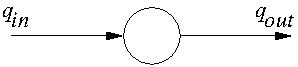
\includegraphics{compartiment}
\caption{Représentation symbolique d'un compartiment}
\label{fig:compartiment}
\end{center}
\end{figure}

Un système à compartiments est constitué par un {\em réseau} de 
compartiments interconnectés et numérotés de $1$ à $n$. Pour fixer
les idées, un exemple de système à $3$ compartiments est représenté
à la figure \ref{fig:exemplecomp}. Les flèches indiquent les flux de
contenu que les divers compartiments peuvent échanger entre eux et avec
l'extérieur du système.

\begin{figure}[ht]
\begin{center}
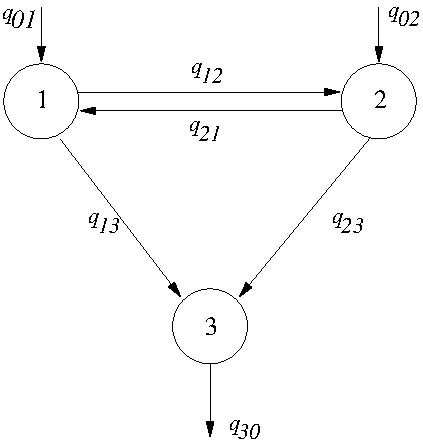
\includegraphics[width=5cm]{exemplecomp}
\caption{Exemple de graphe d'un système à compartiments}
\label{fig:exemplecomp}
\end{center} 
\end{figure}

D'une manière générale, un système à compartiments sera donc 
représenté par un {\em graphe orienté} dont les noeuds correspondent 
aux compartiments et les arcs aux flux. On introduit les notations suivantes~:
\begin{description}
\item $x_i$ désigne la quantité contenue dans le compartiment d'indice $i$,
$(i = 1, ... ,n)$. Cette quantité est toujours {\em positive}. Avec un léger
abus de langage, on
dira aussi pour simplifier que $x_i$ désigne le {\em niveau} du compartiment $i$.
\item $q_{ij}$ désigne le flux circulant du compartiment $i$ vers 
le compartiment $j$, $(i = 1, ... ,n ; j = 1, ... ,n)$. Comme nous l'avons indiqué 
plus haut, c'est une variable qui est aussi toujours {\em positive} par convention.
\end{description}

\begin{definition}{\bf \em Système ouvert ou fermé}

On dit que le système est {\bf ouvert} lorsqu'il existe des possibilités 
d'échange avec l'extérieur du système. Dans ce cas :
\begin{description}
\item $q_{io}$ désigne le flux circulant du compartiment $i$ vers l'extérieur
\item $q_{oi}$ désigne le flux circulant de l'extérieur vers le compartiment $i$
\end{description}
Dans le cas contraire, on dit que le système est {\bf fermé} : $q_{io} = 
q_{oi} = 0$ pour tout $i$. \qed
\end{definition}

\begin{definition}{\bf \em Système connecté aux entrées et sorties}

Un compartiment $i$ est {\it connecté à une sortie} si il y a un chemin $i \rightarrow j \rightarrow k \rightarrow \dots \rightarrow \ell$ partant de ce compartiment et se terminant en un compartiment $\ell$ à partir duquel il y a un flux de sortie $q_{\ell o}$. Le système est {\it complètement connecté aux sorties} (CCS) si chaque compartiment est connecté à une sortie.

Un compartiment $\ell$ est {\it connecté à une entrée} si il y a un chemin $i \rightarrow j \rightarrow k \rightarrow \dots \rightarrow \ell$ jusqu'à ce compartiment et partant d'un compartiment $i$ dans lequel il y a un flux d'entrée $q_{oi}$. Le système est {\it complètement connecté aux entrées} (CCE) si chaque compartiment est connecté à une entrée.  \qed 
\end{definition}


\section{Modèle d'état}
\markboth{ {\bf \hspace*{5mm}Chapitre 4 }\hfill Systèmes
à compartiments} {{ \bf Sec. \thesection} \hfill
Modèles d'état \hspace*{5mm}}

L'équation de bilan de chaque compartiment (appelée aussi équation de
continuité)
\eqnn
\dot{x_i} = \sum_{j=0}^n q_{ji}(t) - \sum_{j=0}^n q_{ij}(t) \hspace{1cm} i=1,...,n
\label{bilan}
\eeqnn
est l'élément de base pour l'établissement du modèle d'état d'un système
à compartiments. Cette équation exprime que la variation, par 
unité de temps,  de la 
quantité contenue dans un
compartiment est la différence entre la somme des
flux (ou débits) entrants et la somme des flux (ou débits) 
sortants. En pratique, bien s\^ur, les flux qui sont structurellement nuls 
ne sont pas explicités dans l'équation (\ref{bilan}).

La mise en équations du modèle d'état d'un système à compartiments
comporte dès lors deux aspects fondamentaux.

Tout d'abord, la structure du graphe associé au système détermine le nombre
et la structure des équations de bilan (\ref{bilan}) ; les variables $x_i$ sont
les variables d'état tandis que l'ordre du modèle est le nombre $n$ de 
compartiments.

Pour compléter le modèle d'état, il faut ensuite exprimer les flux
en fonction des variables d'état et des variables d'entrée :
\eqnn
q_{ij}(x,u)
\eeqnn
où $x$ et $u$ désignent, comme d'habitude, les vecteurs d'état et 
d'entrée. Cette modélisation fera l'objet de la prochaine section.

La forme générale des équations d'état d'un système à compartiments
est alors la suivante :
\eqnn
\dot{x_i} = \sum_{j=0}^n q_{ji}(x,u) - \sum_{j=0}^n q_{ij}(x,u) \hspace{1cm} i=1,...,n \label{eqetcomp}
\eeqnn
Dans ce modèle, le sens physique des variables d'état $x_i$ est clair : ce sont
les quantités contenues dans chaque compartiment. Par contre, les variables
d'entrée $u$ peuvent être de nature très variable selon les applications comme le montreront les exemples qui vont suivre.

Si l'on définit le {\em vecteur des flux} $q(x,u)$ contenant, dans un ordre arbitraire, 
tous les flux $q_{ij}(x,u)$
qui ne sont pas structurellement nuls, on peut écrire aussi le modéle d'état
(\ref{eqetcomp}) sous la forme matricielle plus compacte :
\eqn
\dot{x} = Lq(x,u) \label{modetcomp}
\eeqn
où $L$ est la matrice d'incidence du graphe orienté, dont les coefficients appartiennent tous au triplet
$(-1,0,1)$, qui est .

\begin{exemple}
Pour le système représenté à la figure \ref{fig:exemplecomp}, le
modèle d'état s'écrit :
\eqnn
\dot{x_1} &=& q_{01}(x,u) - q_{12}(x,u) - q_{13}(x,u) + q_{21}(x,u) \\
\dot{x_2} &=& q_{02}(x,u) + q_{12}(x,u) - q_{21}(x,u) - q_{23}(x,u) \\
\dot{x_3} &=& q_{13}(x,u) + q_{23}(x,u) - q_{30}(x,u)
\eeqnn
Si l'on définit le vecteur des flux :
\eqnn
q(x,u) \triangleq \bma{c} q_{01}(x,u) \\ q_{02}(x,u) \\ q_{12}(x,u) \\
q_{13}(x,u) \\ q_{21}(x,u) \\ q_{23}(x,u) \\ q_{30}(x,u) \ema
\eeqnn
le modèle d'état s'écrit sous la forme matricielle (\ref{modetcomp}) avec 
la matrice $L$ :
\eqnn
L \triangleq \bma{ccccccc} 1 & 0 & -1 & -1 & 1 & 0 & 0 \\
0 & 1 & 1 & 0 & -1 & -1 & 0 \\
0 & 0 & 0 & 1 & 0 & 1 & -1 \ema.
\eeqnn
\qed
\end{exemple}

\section{Modélisation des flux}

Selon les applications, les fonctions $q_{ij}(x,u)$ représentant les flux peuvent prendre des formes très variées.  Elles doivent cependant être définies de manière à garantir que le système à compartiments est un {\em système positif} c'est à dire un système dont chaque variable
d'état reste positive le long des trajectoires. C'est une garantie de vraisemblance du modèle puisque les variables d'état représentent des grandeurs qui n'ont pas de sens physique si
elles sont négatives.

\begin{definition} \label{vecpositif} {\bf \em Vecteur positif et orthant positif}

Un vecteur $x = (x_1, \ldots , x_n)^T$ est positif (notation
$x \geq 0$) si chacune de ses composantes est un nombre réel positif~:
$x_i \geq 0$ pour tout $i$.

L'orthant positif de dimension $n$ (noté $\RR_+^n$) est l'ensemble de tous les vecteurs positifs de dimension $n$. \qed
\end{definition}

\begin{definition}{\bf \em Système positif}

Un système dynamique $\dot x=f(x,u)$ est un système positif si, pour toute entrée $u(t)$ admissible, son état
est confiné dans l'orthant positif lorsque l'état initial est positif~:
\eqnn
x(t_0) \in \real_+^n \text{ et } u(t) \in {\cal U}  \Longrightarrow x(t)
\in \real_+^n  \hh \forall t \geq t_0. \qed
\eeqnn
\end{definition}

Le théorème suivant donne une condition suffisante facile à utiliser pour vérifier qu'un système est positif. 

\begin{theoreme} 
Un système dynamique $\dot x=f(x,u)$ est un système positif si $f(x,u)$ est différentiable et si
\eqnn
x \in \real_+^n \;\;\;\; \mbox{et} \;\;\;\; x_i = 0 \;\; \Longrightarrow \;\; \dot x_i \geq 0 \;\;\;\; \forall i. \qed
\eeqnn
\end{theoreme}
Pour garantir qu'un système à compartiments est un système positif, on impose les conditions suivantes aux fonctions de flux $q_{ij}(x,u)$~:
\begin{itemize}
\item[C1.]  Les fonctions $q_{ij}(x,u)$ sont des fonctions positives de leurs arguments sur leur domaine de définition~:
\eqnn
q_{ij}(x,u) : \real^n_+ \times \real^m \rightarrow \real_+
\eeqnn 
\item[C2.] Les fonctions $q_{ij}(x,u)$ sont des fonctions continues et dérivables de leurs arguments sur leur domaine de définition.
\item[C3.]  Comme il ne peut y avoir de flux sortant d'un compartiment vide, les fonctions $q_{ij}(x,u)$ vérifient la condition~:
\eqnn
x_i = 0 \;\; \Rightarrow \;\; q_{ij}(x,u) = 0
\eeqnn
\end{itemize}
\begin{theoreme} 

Sous les conditions C1, C2, C3, un système à compartiments $\dot x = Lq(x,u)$
est un système positif.
\cqfd
\end{theoreme}
\begin{exemple}\label{systhyd}{\bf \em Système hydraulique}

Considérons un système hydraulique formé d'un ensemble 
de réservoirs situés à des altitudes différentes
et dont le contenu liquide s'écoule \og en cascade \gf
des réservoirs les plus élevés vers les réservoirs les plus bas sous l'action
de la gravité. Un exemple est illustré à la figure \ref{Fig:cascade}.
\begin{figure}[h] 
\begin{center}
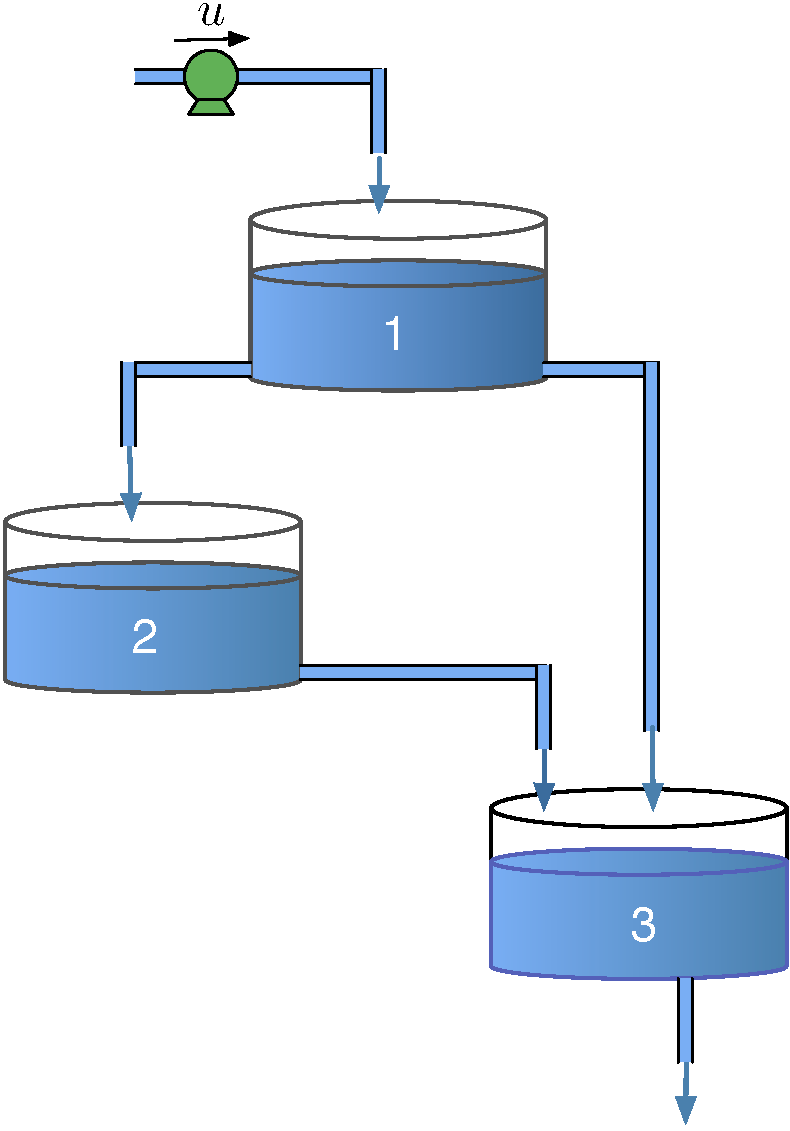
\includegraphics[width=7cm]{cascade}
\caption{Cascade de réservoirs}
\label{Fig:cascade}
\end{center} 
\end{figure}

Il s'agit clairement d'un système à compartiments dont le graphe associé
est représenté à la figure \ref{Fig:grafassoc} et dont les équations de 
continuité s'écrivent~:
\begin{equation*} \begin{split} 
\dot x_1 &= q_{01} - q_{12} - q_{13} \\
\dot x_2 &=  q_{12} - q_{23} \\
\dot x_3 &= q_{13} + q_{23} - q_{30} 
\end{split} \end{equation*}
\begin{figure}[h] 
\begin{center}
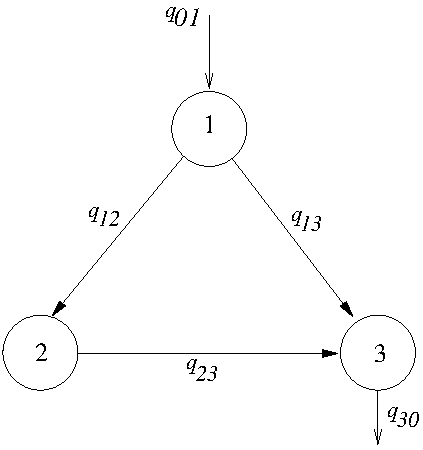
\includegraphics[width=7cm]{grafassoc}
\caption{Graphe associé à la cascade de résevoirs}
\label{Fig:grafassoc}
\end{center} 
\end{figure}
Dans ces équations, les variables d'état $x_1$,$ x_2$ et $x_3$ désignent 
évidemment les volumes d'eau contenus dans les réservoirs et les flux 
$q_{ij}$ représentent les débits s'écoulant des réservoirs supérieurs
vers les réservoirs inférieurs. Pour compléter le modèle, il faut 
exprimer ces flux en fonction des variables d'état et de signaux d'entrée
convenablement choisis.
Le débit fourni par la
pompe d'alimentation du réservoir supérieur peut clairement être choisi
comme variable d'entrée. Le débit de sortie $q_{ij}$
de chaque réservoir est une fonction positive du volume $x_i$ du réservoir. La forme de cette fonction dépend de la forme du réservoir et de la configuration de l'orifice par lequel l'eau s'écoule. Considérons le cas où les réservoirs sont de section horizontale constante et où l'écoulement s'effectue par un orifice rectangulaire situé au bas des réservoirs. La hauteur de l'eau dans un réservoir est notée~:
\eqnn
h_i = \frac {x_i}{S_i}
\eeqnn
où $S_{i}$ désigne la section du réservoir.
Selon les lois de l'hydraulique, nous savons que, lorsque la hauteur de l'eau $h_i$ est grande par rapport à la hauteur de l'orifice, la relation entre le débit et la hauteur d'eau est proportionnelle à $\sqrt{h_i}$ (loi de Torricelli~\footnote{Cette loi énoncée par Torricelli en 1643 énonce que la vitesse $v$ de l'eau à la sortie d'un réservoir de hauteur $h$ vérifie $v^2=2gh$. Elle se démontre intuitivement par analogie avec un corps en chute libre: un volume élémentaire d'eau à la surface du réservoir transforme son énergie potentielle $\rho g h$ en énergie cinétique $\rho v^2/2$ quand il arrive à la sortie du réservoir, où $\rho$ désigne la masse volumique. Plus rigoureusement, on la déduit du théorème de Bernoulli sans perte de charge ou pompe $p+\rho gz +\rho v^2/2 = \mathrm{constante}$, où $p$ désigne la pression et $z$ l'altitude.}). Par contre lorsque la hauteur de l'eau est inférieure à la hauteur de l'orifice, le débit devient proportionnel à $h_i\sqrt{h_i}$ (loi de l'écoulement pour un déversoir de forme rectangulaire). On peut dès lors proposer un modèle de la forme~:
\eqnn
q_{ij} = \frac { \alpha_{ij}h_i\sqrt{h_i} }{ \beta_{ij} + h_i}
\eeqnn
où $ \alpha_{ij}$ et $ \beta_{ij}$ sont des constantes positives. En effet ce modèle vérifie bien la propriété que pour de faibles hauteurs d'eau ($h_i \ll \beta_{ij}$), le débit $q_{ij}$ est proportionnel à $h_i\sqrt{h_i}$ tandis que pour des hauteurs d'eau élevées ($h_i \gg \beta_{ij}$), le débit $q_{ij}$ est proportionnel à $\sqrt{h_i}$.
On peut exprimer $q_{ij}$ en fonction de $x_i$~:
\eqnn
q_{ij}(x_i) = \frac {k_{ij}x_i\sqrt{x_i} }{S_i \beta_{ij} + x_i} \hh \mbox{ avec } k_{ij} \triangleq \frac{\alpha_{ij}}{\sqrt{S_i}} 
\eeqnn
Alors le modèle d'état s'écrit finalement~:
\begin{equation} \begin{split} \label{modetacasca}
\dot x_1 &= - \frac {k_{12}x_1\sqrt{x_1} }{S_1\beta_{12} + x_1} - \frac {k_{13}x_1\sqrt{x_1} }{S_1 \beta_{13} + x_1} + u, \\
\dot x_2 &=  \frac {k_{12}x_1\sqrt{x_1} }{S_1 \beta_{12} + x_1} - \frac {k_{23}x_2\sqrt{x_2} }{S_2 \beta_{23} + x_2},
\\
\dot x_3 &= \frac{k_{13}x_1\sqrt{x_1} }{S_1 \beta_{13} + x_1} + \frac {k_{23}x_2\sqrt{x_2} }{S_2 \beta_{23} + x_2} -
\frac {k_{30}x_3\sqrt{x_3} }{S_3 \beta_{30} + x_3}.
\end{split} \end{equation}
On observe que les fonctions $q_{ij}(x_{i})$ vérifient bien les conditions de positivité C1, C2, C3. \qed
\end{exemple}

\section{Modèles linéaires avec commande par les alimentations 
extérieures}

C'est la classe de modèles à compartiments que l'on rencontre le plus
couramment dans la littérature. Elle est caractérisée par les définitions
suivantes des flux~:
\begin{enumerate}
\item Les flux entre compartiments et les flux de sortie du système sont 
des fonctions linéaires du
niveau du compartiment donneur :
\eqnn
q_{ij} = k_{ij}x_i \hspace{1cm} k_{ij} > 0 \hspace{1cm} (i=1,...,n;j=0,...,n)
\eeqnn
\item Les entrées $u_{\ell}$ du système sont proportionnelles aux flux
d'alimentation~: 
\eqnn
q_{0\ell} = k_{0\ell}u_{\ell} 
\eeqnn
\end{enumerate}
Dans ce cas, l'information nécessaire à l'écriture du modèle d'état 
est entièrement contenue dans le graphe du système. Le modèle d'état
prend la forme générale d'un système linéaire (voir chapitre 1), c-à-d~:
\eqnn
\dot{x} = Ax + Bu
\eeqnn
mais avec les particularités structurelles suivantes~:
\begin{enumerate}
\item La matrice $A$ est une {\em matrice de Metzler} c-à-d  telle que $a_{ij} 
\geq 0$ 
pour tout $i \neq j$
\item La matrice $A$ est diagonalement dominante c-à-d
\eqnn
|a_{ii}| \geq \sum_{j \neq i} a_{ji} 
\eeqnn
\item La matrice $B$ est une {\em matrice élémentaire} de plein rang, c'est à
dire une matrice qui contient au plus un élément non nul par ligne et par
colonne.
\end{enumerate}

\begin{exemple}

Le modèle d'état linéaire du système à compartiments
correspondant au graphe de la figure \ref{fig:exemplecomp} 
s'écrit comme suit~:
\begin{equation} \begin{split}
\bma{c} \dot x_1 \\ \dot x_2 \\ \dot x_3 \ema &= 
\bma{ccc} -(k_{12} + k_{13}) & k_{21} & 0 \\ 
k_{12} & -(k_{21} + k_{23}) & 0 \\ k_{13} & k_{23} & - k_{30} \ema
\bma{c} x_1 \\ x_2 \\ x_3 \ema \\ &\hd
+ \bma{cc} k_{01} & 0 \\ 0 & k_{02} \\ 0 & 0 \ema
\bma{c} u_1 \\ u_2 \ema
\end{split} \end{equation}
On observe que $A$ est bien une matrice de Metzler diagonalement
dominante et que $B$ est une matrice élémentaire de plein rang ($= 2$).
\cqfd
\end{exemple}

\begin{exemple}{\bf \em Modélisation physiologique}

Les physiologistes s'intéressent souvent à décrire et à analyser la 
propagation de substances biologiques ou chimiques dans le corps des
mammifères. Il peut s'agir de substances médicamenteuses (on parle alors
d'études pharmacocinétiques) ou encore de substances toxiques absorbées
volontairement ou accidentellement. Il peut s'agir aussi de substances d'origine
naturelle telle que des hormones ou des protéines. Les modèles à 
compartiments sont fréquemment utilisés pour procéder à de telles 
études : le corps du mammifère est alors représenté par un ensemble
plus ou moins diversifié de réservoirs interconnectés. 

Considérons l'exemple
de la figure \ref{Fig:grapharmaco}.
\begin{figure}[ht] 
\begin{center}
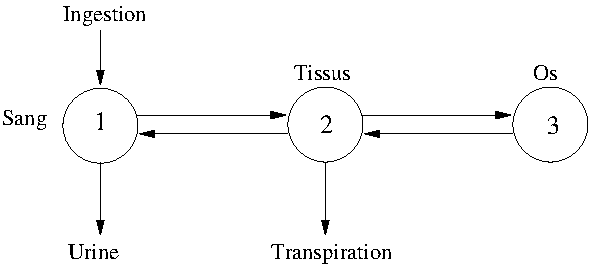
\includegraphics{grapharmaco}
\caption{Graphe d'un modèle à compartiments en pharmacocinétique}
\label{Fig:grapharmaco}
\end{center} 
\end{figure}
Une substance toxique (par exemple du plomb) est ingérée par un animal et
pénêtre dans le sang. Cette substance  se propage progressivement
dans le corps, passant du sang vers les tissus tout d'abord, vers les os ensuite.
Elle est excrétée par la transpiration d'une part et par les voies urinaires
d'autre part. Le modèle à compartiments linéaires correspondant
au graphe de la figure \ref{Fig:grapharmaco} est le suivant :
\begin{equation*} \begin{split}
\bma{c} \dot x_1 \\ \dot x_2 \\ \dot x_3 \ema &= 
\bma{ccc} -(k_{10} + k_{12}) & k_{21} & 0 \\ 
k_{12} & -(k_{20} + k_{21} + k_{23}) & k_{32} \\ 0 & k_{23} & - k_{32} \ema
\bma{c} x_1 \\ x_2 \\ x_3 \ema \\
& \hd + \bma{c} k_{ 01}\\ 0 \\ 0 \ema u.
\end{split} \end{equation*}
Dans ce modèle, les variables d'état $x_1$, $x_2$ et $x_3$ désignent
bien s\^ur les quantités de substance toxique dans les trois compartiments
(sang, tissus et os). La variable d'entrée $u$ désigne le flux d'ingestion 
par le corps.
\cqfd
\end{exemple}

\section{Modèles non linéaires avec commande par les flux}

Nous considérons maintenant des systèmes non linéaires à compartiments
dont les flux
$q_{ij}$ peuvent être des fonctions non linéaires quelconques de
leurs arguments satisfaisant les conditions C1 - C3. Nous avons déjà rencontré
un modèle non linéaire dans l'exemple de la cascade de
réservoirs. Toutefois, dans cet exemple, les flux entre 
compartiments n'étaient pas fonction des variables d'entrée $u_{\ell}$. Ici nous
considérerons le cas où certains flux entre compartiments sont des fonctions
explicites de variables d'entrée $u_{\ell}$ qui permettent de contr\^oler le débit
passant entre ces compartiments.  On utilise la représentation
symbolique de la figure
\ref{Fig:contflux} pour indiquer la présence d'une telle variable de contr\^ole.
\begin{figure}[ht] 
\begin{center}
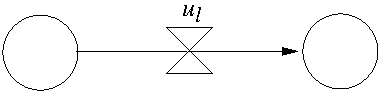
\includegraphics{contflux}
\caption{Représentation symbolique d'un flux contr\^olé}
\label{Fig:contflux}
\end{center} 
\end{figure}

\begin{exemple}{\bf \em Réseau de réservoirs}

Considérons le système hydraulique illustré à la figure \ref{Fig:reseauh}. Ce
réseau de réservoirs est celui de l'exemple de la cascade de
réservoirs (exemple \ref{systhyd}) que nous avons rencontré
précédemment, mais avec une petite modification~: l'écoulement entre le
réservoir $2$ et le réservoir $3$ n'est plus un écoulement libre mais est devenu
un écoulement forcé par la pompe. Dans la mesure où cette pompe est
commandable, il est naturel de considérer le débit pompé $F$ comme une variable
d'entrée. 

\begin{figure}[h] 
\begin{center}
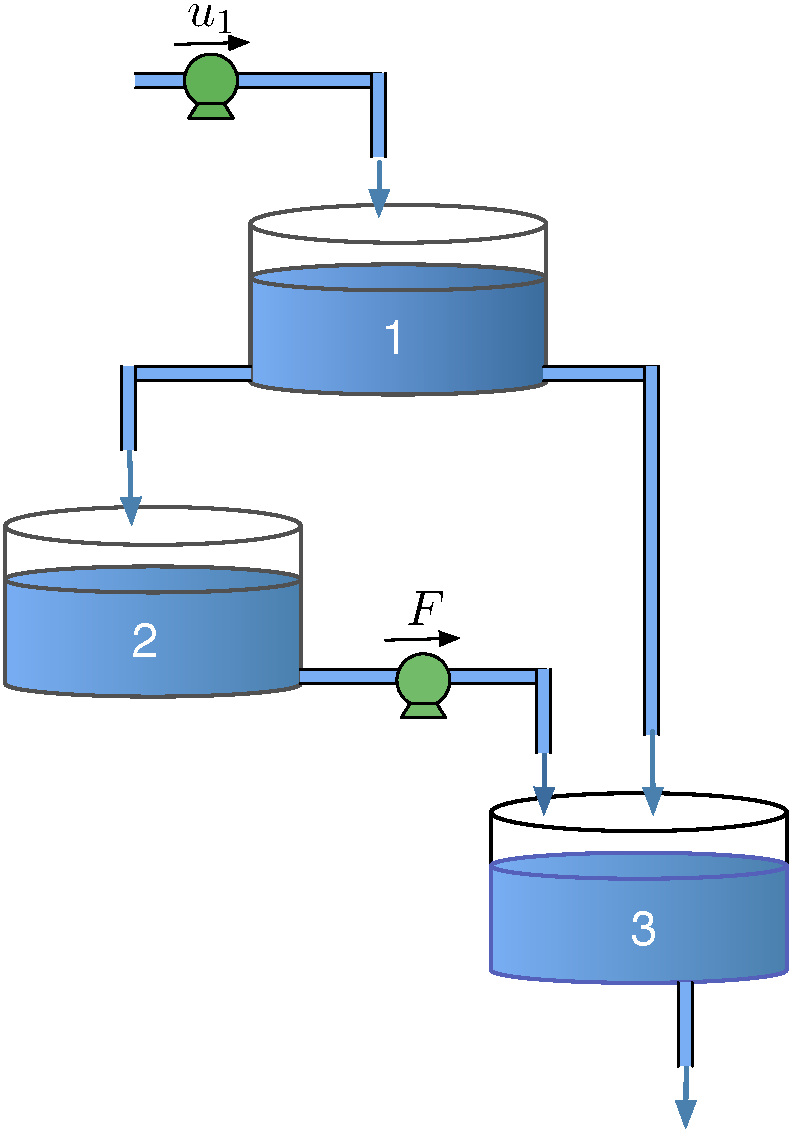
\includegraphics[width=7cm]{reseauh}
\caption{Réseau de réservoirs}
\label{Fig:reseauh}
\end{center} 
\end{figure}

Le modèle d'état (\ref{modetacasca}) que nous avions obtenu pour la cascade de
réservoirs est alors simplement modifié comme suit~:
\begin{equation} \begin{split}
\dot x_1 &= - q_{12}(x_1) - q_{13}(x_1) + u_1 \\
\dot x_2 &=  q_{12}(x_1) - u_2 \label{modres1} \\
\dot x_3 &= q_{13}(x_1) - q_{30}(x_3) + u_2 
\end{split} \end{equation}
où les variables d'état $x_i$ sont les volumes d'eau contenus dans les
réservoirs, la variable d'entrée $u_1$ est le débit d'alimentation du premier
réservoir, la variable d'entrée $u_2 = F$ est le débit pompé du deuxième 
vers le troisième  réservoir et les fonctions $q_{ij}(x_i)$ sont définies comme suit~:
\eqnn
q_{ij}(x_i) = \frac {k_{ij}x_i\sqrt{x_i} }{S_i \beta_{ij} + x_i}
\eeqnn
On observe que ce modèle d'état {\it ne peut pas} être celui d'un système à
compartiments vérifiant les conditions C1 - C3. En effet le flux $q_{23} = u_2$ ne vérifie pas la condition C3 et le système n'est pas positif : une simulation de ce modèle peut
conduire à des niveaux négatifs dans les réservoirs (même si les débits
pompés restent positifs) ce qui est évidemment contradictoire avec la réalité
physique. La difficulté provient du fait que, avec le modèle tel qu'il est écrit, on
peut pomper de l'eau dans le deuxième réservoir même quand il est vide !

On contourne aisément cette difficulté si on modélise le flux $q_{23}$ (qui est le
débit pompé $F$) de manière à respecter la réalité physique et à satisfaire la
condition C3 comme ceci~:
$$
q_{23}(x_2,u_2) = \phi(x_2)u_2
$$
où $\phi(x_2)$ est une fonction positive vérifiant $\phi(0) = 0$ et
$u_2$ représente l'actionnement de la pompe. On obtient alors un système à
compartiments dont le graphe est présenté à la figure \ref{Fig:graphreseau} et
dont le modèle d'état s'écrit~:
\begin{equation*} \begin{split}
\dot x_1 &= - q_{12}(x_1) - q_{13}(x_1) + u_1 \\
\dot x_2 &=  q_{12}(x_1) - \phi(x_2)u_2 \\
\dot x_3 &= q_{13}(x_1) - q_{30}(x_3) + \phi(x_{2})u_2 
\end{split} \end{equation*}
\begin{figure}[h] 
\begin{center}
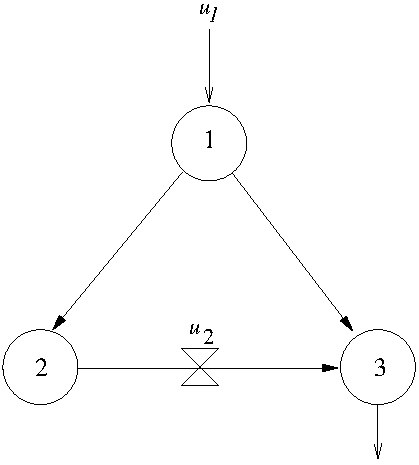
\includegraphics[width=7cm]{graphreseau}
\caption{Graphe associé au réseau de réservoirs}
\label{Fig:graphreseau}
\end{center} 
\end{figure}
\cqfd
\end{exemple}

La propriété structurelle fondamentale des systèmes linéaires à
compartiments se généralise aux systèmes non linéaires de la manière
suivante.
\begin{theoreme} 

Soit un système non linéaire à compartiments dont les flux $q_{ij}$ vérifient les
conditions C1 - C3. Alors les flux peuvent s'écrire de la fa\c con suivante~:
\eqnn
&& q_{ij}(x,u) = a_{ij}(x,u)x_i \hspace{4mm}
(i=1,...,n;j=1,...,n)\\ 
&& q_{i0}(x,u) = a_{i0}(x,u)x_i \hspace{4mm}
(i=1,...,n)\\
&& q_{0i} = k_{0i}u_i
\eeqnn
où les fonctions $a_{ij}(x,u)$ et $a_{i0}(x,u)$, définies sur
l'orthant positif, sont continues. 

En conséquence, le modèle d'état du système peut se mettre sous la forme
suivante~:
$$
\dot x = A(x,u)x + Bu
$$
où la matrice $A(x,u)$ est une matrice de Metzler diagonalement dominante pour
tout $(x,u)$ dans l'orthant positif et $B$ est une matrice élémentaire.
\cqfd
\end{theoreme}
Nous terminons ce chapitre par la présentation d'un autre exemple industriel
classique de système à compartiments.
\begin{exemple}{\bf \em Procédé de distillation binaire}

Un procédé de distillation binaire est un procédé utilisé pour séparer un
mélange de deux composés chimiques, sous forme liquide, appelé {\em charge}. Un {\it
dépropaniseur} ayant pour fonction de séparer le propane du butane est un
exemple typique de procédé de distillation binaire dans l'industrie pétrochimique.

La séparation s'effectue par évaporation dans une enceinte fermée appelée {\em ballon} (voir figure \ref{Fig:distillation}).
\begin{figure}[h]
\begin{center}
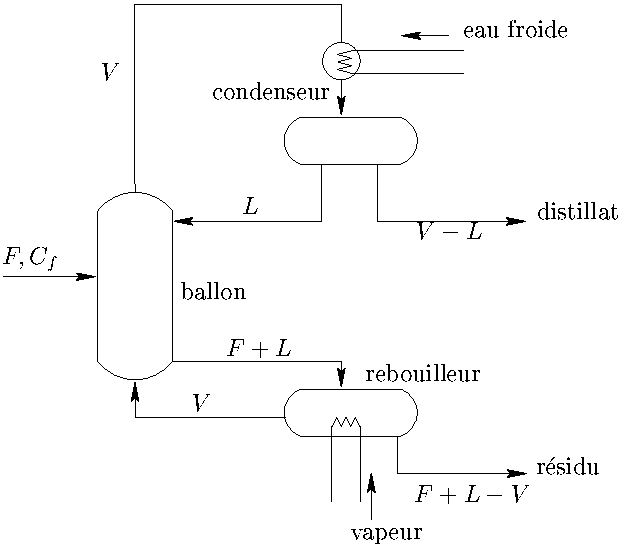
\includegraphics[width=8cm]{proc_distil}
\caption{Procédé de distillation}
\label{Fig:distillation}
\end{center} 
\end{figure}
Au sommet du ballon sort le {\it distillat} contenant essentiellement le composé léger avec
un peu de composé lourd. Au fond du ballon sort le {\it résidu} qui contient
essentiellement le composé lourd avec un peu de composé léger. Le ballon est alimenté par la charge avec un débit molaire $F$ (mol/min). Le flux de vapeur sortant au sommet du ballon est refroidi et complètement condensé. Le liquide
sortant du condenseur est partiellement recyclé vers le ballon avec un débit
molaire $L$. Le reste, appelé {\it distillat}, est extrait du système. En fond de
ballon, le liquide sortant est
réchauffé dans un rebouilleur et la vapeur ainsi produite est recyclée dans le ballon.  Le reste, appelé {\it résidu}, est extrait.

On présente ci-dessous un modèle simplifié de la dynamique de ce procédé de distillation en faisant les
hypothèses de modélisation suivantes~:
\begin{enumerate}
\item la charge est liquide et à sa température de bulle;
\item les phases liquide et vapeur dans le ballon et le rebouilleur sont homogènes et à
l'équilibre;
\item dans le ballon la pression est constante et il n'y a pas d'accumulation de vapeur; cette hypothèse permet d'omettre les dépendances en pression dans les équations et implique que le débit de vapeur $V$  à la sortie du ballon est égal au débit à l'entrée; 
\item les débits d'extraction liquide sont ajustés de manière que les masses molaires totales de la phase liquide dans les trois récipients soient constantes : le distillat est donc extrait avec un débit molaire $V-L$, le liquide en fond de ballon avec un débit molaire $F+L$ et le résidu avec un débit molaire $F+L-V$. Evidemment, cela implique que l'inégalité $0 < L < V < F+L$ soit vérifiée.\\
\end{enumerate}
Ainsi décrit, le procédé de distillation peut être vu comme un système à
compartiments dont le modèle dynamique est constitué des
équations de bilan de l'un des deux composés dans le ballon, dans le condenseur et dans le rebouilleur. Le graphe de ce système à
compartiments est présenté à la figure \ref{Fig:graphdisti} et les équations
d'état sont les suivantes~:
\begin{equation*} \begin{split}
\dot x_1 &= u_2 k(x_2) - u_{1}\frac{x_1}{m_1} - (u_2 - u_1) \frac{x_1}{m_1}\\
\dot x_2 &= u_1\frac{x_1}{m_1} - (u_1+u_3)\frac{x_2}{m_2} + u_2(k(x_3) - k(x_2)) + u_3c_f\\
\dot x_3 &= (u_1 + u_3)(\frac{x_2}{m_2} - \frac{x_3}{m_3}) + u_2(\frac{x_3}{m_3} - k(x_3))
\end{split} \end{equation*}
\begin{figure}[h]
\begin{center}
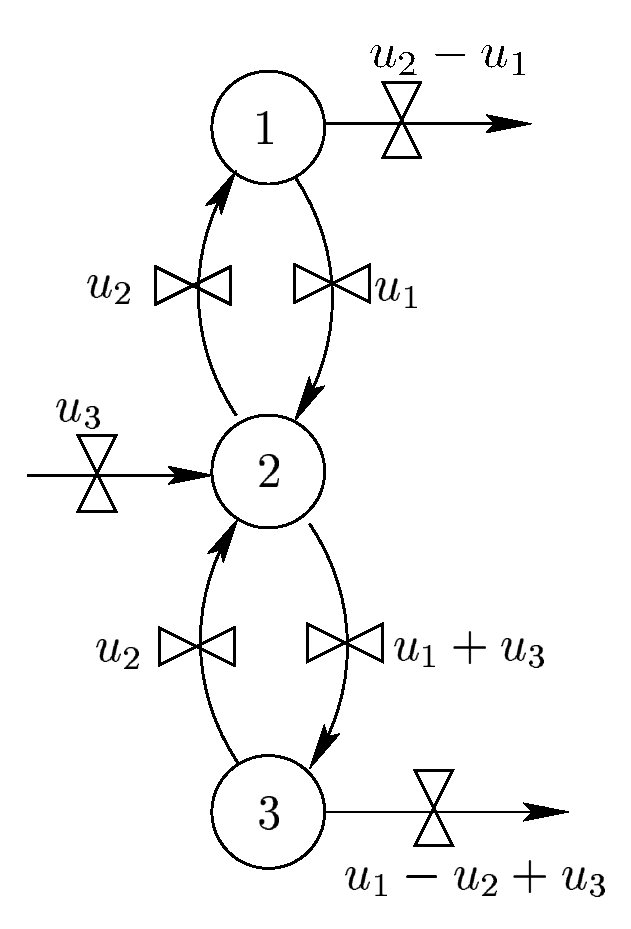
\includegraphics[width=5cm]{graphprocdistil}
\caption{Graphe associé au procédé de distillation}
\label{Fig:graphdisti}
\end{center} 
\end{figure}
Dans ces équations, les variables d'état $x_i$ représentent la masse molaire du
composant léger dans la phase liquide du condenseur (indice $1$), du ballon (indice $2$) et du rebouilleur (indice  $3$); les paramètres $m_i$ sont les 
masses molaires totales (et constantes) correspondantes : le rapport $x_i/m_i$ est la {\it fraction molaire}; le paramètre $c_f$
est la fraction molaire du composé léger dans la charge; les variables d'entrées $u_1 =
L$, $u_2 = V$ et
$u_3 = F$ sont, respectivement, les débits molaires de reflux, de production de vapeur et
d'alimentation. Enfin, la fonction $k(x)$ est une relation d'équilibre
liquide-vapeur permettant de relier la fraction molaire du composant léger quittant le liquide
sous forme vapeur à la fraction molaire du composant dans la phase liquide. 
\begin{figure}[ht]
\begin{center}
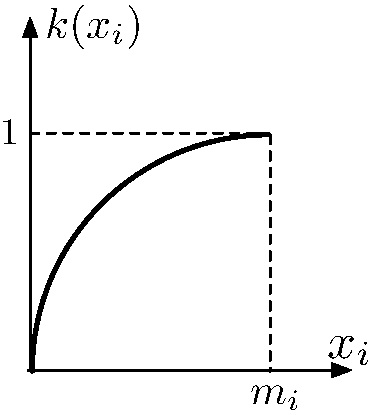
\includegraphics[width=4cm]{separ}
\caption{Relation d'équilibre liquide-vapeur}
\label{Fig:separ}
\end{center} 
\end{figure}

\noindent Cette
relation s'exprime classiquement comme suit~:
\eqnn
k(x_i) \triangleq \frac{\alpha x_i}{m_i + (\alpha - 1)x_i}
\eeqnn
où le paramètre constant $\alpha > 1$ porte le nom de facteur de séparation.
Cette fonction, définie sur l'intervalle $[0,m_i]$, vérifie $k(0) = 0$ et
$k(m_i) = 1$ (voir figure \ref{Fig:separ}). \qed  
\end{exemple}

\section{Exercices}

\begin{exercice}{\bf \em Un système à compartiments}

Soit le système dynamique suivant:
\begin{align*}
\dot x_{1} &= x_{3} - \log (1+x_{1}) \\
\dot x_{2} &= x_{3} - x_{2}^2 \\
\dot x_{3} &= x_{2}^2 - 2x_{3} + u
\end{align*}
Démontrer qu'il s'agit d'un système à compartiments. Dessiner le graphe associé. Calculer les flux $q_{ij}$, la matrice $L$ et la matrice $A(x,u)$. \qed
\end{exercice}
\vv

\begin{exercice}{\bf \em Un système hydraulique}

Un système hydraulique comportant trois réservoirs et deux pompes
est représenté à la figure \ref{Fig:systhydr}.
\begin{figure}[h]
\begin{center}
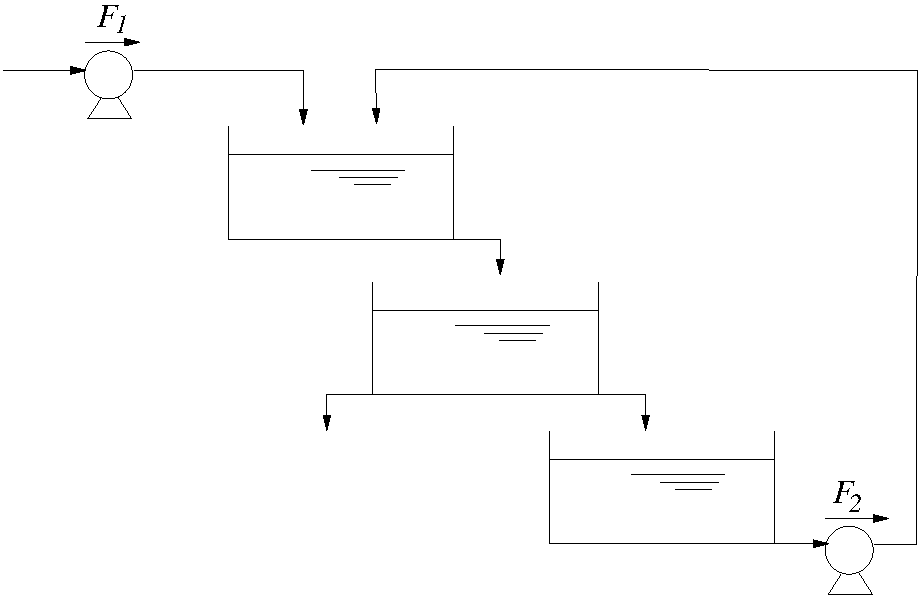
\includegraphics[width=8cm]{systhydr}
\caption{Système hydraulique}
\label{Fig:systhydr}
\end{center} 
\end{figure}
\begin{enumerate}
\item Etablir un modèle d'état du système en considérant les
débits volumétriques $u_1 = F_1$ et $u_2 = F_2$ comme variables
d'entrée. Montrer que le système obtenu n'est {\it pas} un système
positif. 
\item Proposer une autre définition de la variable d'entrée $u_2$ qui
garantisse que le système soit positif. 
\item Dessiner le graphe du modèle à compartiments ainsi obtenu. \qed
\end{enumerate}
\end{exercice}
\vv 

\begin{figure}[!ht] 
\begin{center}
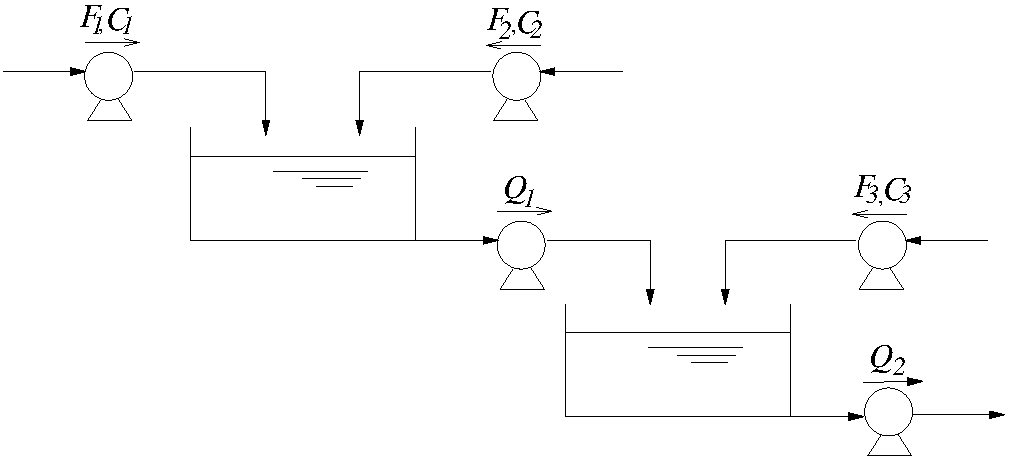
\includegraphics[width=8cm]{cuvmel}
\caption{Réseau de cuves de mélange}
\label{Fig:cuvmel}
\end{center} 
\end{figure}

\begin{exercice}{\bf \em Un réseau de cuves de mélange}

Le système représenté à la figure \ref{Fig:cuvmel} est con\c cu pour
mélanger trois substances $X_1, X_2, X_3$ dont les concentrations
d'alimentation sont notées $C_1, C_2, C_3$. Les volumes contenus
dans les deux cuves sont notés $V_1, V_2$. Les débits volumétriques
des pompes sont notés $Q_1, Q_2, F_1, F_2, F_3$.

\begin{enumerate}
\item Etablir un modèle d'état du système avec les variables
d'entrée suivantes~: $u_1 = Q_1/V_1, u_2 = Q_2/V_2, u_3 = C_1, u_4 =
C_2, u_5 = C_3$. Les débits $F_i$, $i = 1, \dots , 3$, sont supposés
constants.
\item Justifier la forme des variables d'entrées $u_1$ et $u_2$. \qed
\end{enumerate}
\end{exercice}
\vv

\begin{exercice}{\bf \em Modèle linéaire à compartiments}

Caractériser la structure du graphe d'un modèle linéaire à
compartiments dont la matrice $A$ est~:
\begin{enumerate}
\item bidiagonale
\item tridiagonale
\item triangulaire inférieure \qed
\end{enumerate}
\end{exercice}
\vv

\begin{exercice}{\bf \em Modèle du  procédé de distillation}

Déterminer la matrice $A(x,u)$ du modèle du procédé de distillation. \qed
\end{exercice}
\vv

\begin{exercice}{\bf \em Des réservoirs communicants}

Un système à deux réservoirs communicants est représenté à la
figure \ref{Fig:reservoircom} Le liquide s'écoule librement entre les deux
réservoirs et vers l'extérieur sous l'action de la pression hydrostatique.

\begin{figure}[h]
\begin{center}
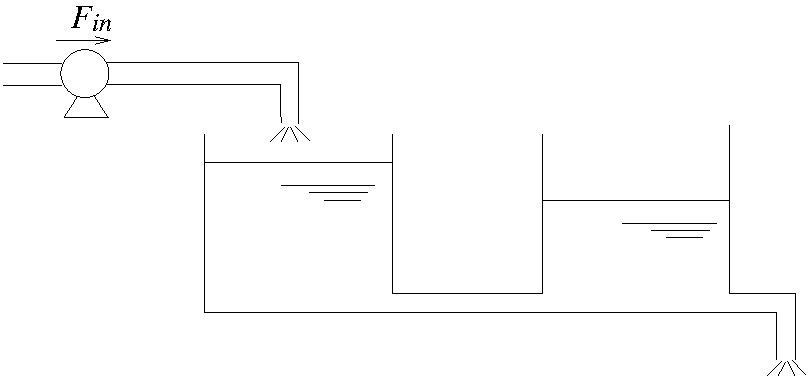
\includegraphics[width=8cm]{reservoircom}
\caption{Réservoirs communicants}
\label{Fig:reservoircom}
\end{center} 
\end{figure}

\begin{enumerate}
\item Etablir un modèle d'état du système. Le débit fourni par la
pompe d'alimentation est la seule variable d'entrée du système.
\item Montrer qu'il s'agit d'un système à compartiments. Dessiner le
graphe associé. Expliciter les flux entre compartiments. \qed
\end{enumerate}
\end{exercice}


\end{document}
